%%%% ijcai21.tex

\typeout{IJCAI--21 Instructions for Authors}

% These are the instructions for authors for IJCAI-21.

\documentclass{article}
\pdfpagewidth=8.5in
\pdfpageheight=11in
% The file ijcai21.sty is NOT the same than previous years'
\usepackage{ijcai21}
% Use the postscript times font!
\usepackage{times}
\usepackage{soul}
\usepackage{url}
\usepackage[hidelinks]{hyperref}
\usepackage[utf8]{inputenc}
\usepackage[small]{caption}
\usepackage{graphicx}
\usepackage{amsmath}
\usepackage{amsthm}
\usepackage{booktabs}
\usepackage{algorithm}
\usepackage{algorithmic}
\urlstyle{same}


% the following package is optional:
%\usepackage{latexsym}

% See https://www.overleaf.com/learn/latex/theorems_and_proofs
% for a nice explanation of how to define new theorems, but keep
% in mind that the amsthm package is already included in this
% template and that you must *not* alter the styling.
\newtheorem{example}{Example}
\newtheorem{theorem}{Theorem}

% Following comment is from ijcai97-submit.tex:
% The preparation of these files was supported by Schlumberger Palo Alto
% Research, AT\&T Bell Laboratories, and Morgan Kaufmann Publishers.
% Shirley Jowell, of Morgan Kaufmann Publishers, and Peter F.
% Patel-Schneider, of AT\&T Bell Laboratories collaborated on their
% preparation.

% These instructions can be modified and used in other conferences as long
% as credit to the authors and supporting agencies is retained, this notice
% is not changed, and further modification or reuse is not restricted.
% Neither Shirley Jowell nor Peter F. Patel-Schneider can be listed as
% contacts for providing assistance without their prior permission.

% To use for other conferences, change references to files and the
% conference appropriate and use other authors, contacts, publishers, and
% organizations.
% Also change the deadline and address for returning papers and the length and
% page charge instructions.
% Put where the files are available in the appropriate places.

%PDF Info Is REQUIRED.
\pdfinfo{
/TemplateVersion (IJCAI.2021.0)
}

\title{Utilização de Métodos de Aprendizado de Máquina na Classificação de Imagens para
Reconhecimento de Lixo Orgânico ou Reciclável}

% Single author syntax
\author{
    Antônio Marcos Machado, Bárbara Boechat, Bruce Williss, Elvis Ribeiro
    \affiliations
    Universidade Federal de São João del-Rei
    \emails
}

% Multiple author syntax (remove the single-author syntax above and the \iffalse ... \fi here)
% Check the ijcai21-multiauthor.tex file for detailed instructions
\iffalse
\author{
Antônio Marcos Machado$^1$
\and
Bárbara Boechat$^2$\and
Bruce Willis$^{2,3}$\And
Elvis Ribeiro$^4$

\affiliations
$^1$UFSJ\\
$^2$UFSJ\\
$^3$UFSJ\\
$^4$UFSJ
\emails
\{barbs.boechat, elvishribeiro, amm.bernardes, bruce.ufsj\}@gmail.com,
}
\fi

\begin{document}

\maketitle

%%%% Tópicos que o artigo deve conter %%%%%%%
%Título relacionado ao tema do trabalho e identificação dos autores. 
%− Introdução:  que  descreva  o  problema  de  aprendizado  de  máquina,  visões,  etapas  e 
%diferentes abordagens. 
%− Fundamentação teórica: que forneça base sobre aprendizado supervisionado, os 
%algoritmos  envolvidos  nos  experimentos  e  suas  características  específicas  (quando  são 
%adequados, quando não são, vantagens e desvantagens); 
%− Desenvolvimento  do  trabalho  e  análise  de  resultados:  explique  sobre  a  base  utilizada,  a 
%escolha dos atributos e apresente os resultados obtidos pelos classificadores, comparando 
%os  algoritmos  e  destacando  as  características  individuais  de  cada  um  que  podem  ter 
%influenciado nos resultados. 
%− Finalmente, as conclusões e referências


% Comparação de algoritmos de AM na tarefa de classificar 
% imagens de lixo ôrganico ou reciclável
\begin{abstract}
  The {\it IJCAI--21 Proceedings} will be printed from electronic
  manuscripts submitted by the authors. The electronic manuscript will
  also be included in the online version of the proceedings. This paper
  provides the style instructions.
\end{abstract}

\section{Introduction}

Introdução ainda não disponível neste checkpoint.

\section{Fundamentação Teórica}

\subsection{Classificação de Imagens}
%breve levantamento sobre e como funciona o algoritmo
A classificação de imagens é o processo de categorizar e rotular vetores em uma imagem (grupos de pixels) com base em regras específicas, as quais podem se basear em uma ou mais características espectrais, ou texturais. A classificação pode ser feita através de dois métodos gerais os "supervisionados" e "não supervisionados". %Neste trabalho é utilizado o método supervisionado

\subsubsection{Classificação Não Supervisionada}

O método não supervisionado é totalmente automatizado sem o uso de dados de treinamento. Utilizando um algoritmo adequado, as características especificadas de uma imagem são detectadas sistematicamente durante o estágio de processamento da imagem. Estes métodos descrevem um modelo de ‘agrupamento de imagens’ ou ‘reconhecimento de padrões’, os algoritmos ‘ISODATA’ e ‘K-mean’ são comumente utilizados.

\subsubsection{Classificação Supervisionada}

O método supervisionado é o processo de selecionar amostras visualmente nas imagens dos dados de treinamento e atribuí-las a categorias pré-selecionadas dependendo da base de dados utilizada, essas categorias podem ser, por exemplo estradas, edifícios, corpo d'água, vegetação e entre outras, de modo a criar medidas estatísticas a serem aplicadas à imagem inteira. 

'Máxima verossimilhança' e 'distância mínima' são dois métodos comuns para categorizar a imagem inteira usando os dados de treinamento. Por exemplo, a classificação de 'probabilidade máxima' usa as características estatísticas dos dados, onde os valores de média e desvio padrão de cada índice espectral e textural da imagem são calculados primeiro. Então, considerando uma distribuição normal para os pixels em cada classe e usando algumas estatísticas clássicas e relações probabilísticas, a probabilidade de cada pixel pertencer a classes individuais é calculada. Finalmente, os pixels são rotulados para uma classe de recursos que mostram a maior probabilidade

\subsection{Processamento de Imagens}
\label{sub:process_img}
O banco de imagens necessitou da etapa de pré-processamento antes da etapa seguinte de extração de dados e classificação. Assim, foram realizados três tratamentos diferentes, o redimensionamento, o histograma de equalização e a representação das imagens em escalas de cinza, a seguir em \ref{sub:redm}, \ref{sub:histE}  e \ref{sub:gray} mais detalhes sobre os métodos.

\begin{enumerate}
    \item \label{sub:redm} \textbf{Redimensionamento:} Imagens com resoluções elevadas podem causar lentidão no processado caso sejam usadas em seus estados originais, então foi necessário realizar um redimensionamentos para que as imagens passagem a ter resolução de 150x150;
    \item \label{sub:histE} \textbf{Histograma de Equalização:} O histograma é utilizado para fornecer a ideia geral de como é uma imagem, então, a partir disso é possível tentar equalizar uma imagem que aparentemente esteja escura, ou seja, imagem que tenha pixels com valores baixos no histograma, ou que seus pixels tenham valores elevados no histograma, indicando uma imagem muito clara. É ideal equalizar os valores dos pixels com o objetivo de uniformemente espalhar seus níveis e obter como resultado uma melhora no contraste da imagem;
    \item \label{sub:gray} \textbf{Escalas de Cinza:} A conversão da imagem colorida em escala de cinza costuma ser um requisito importante no processamento de imagens e tem como objetivo usar o número limitado de níveis de cinza para preservar a maior quantidade possível do contraste da imagem original. A intensidade do nível de cinza está normalmente no intervalo \([0, 2^b - 1]\), tal que b é o número de bits por pixel.
\end{enumerate}

\subsection{SVM}
%breve levantamento sobre e como funciona o algoritmo
Uma máquina de vetores de suporte (SVM, do inglês: support vector machine) é um conceito na ciência da computação para um conjunto de métodos de aprendizado supervisionado que analisam os dados e reconhecem padrões, usado para classificação e análise de regressão. O SVM padrão toma como entrada um conjunto de dados e prediz, para cada entrada dada, qual de duas possíveis classes a entrada faz parte, o que faz do SVM um classificador linear binário não probabilístico. 

Dados um conjunto de exemplos de treinamento, cada um marcado como pertencente a uma de duas categorias, um algoritmo de treinamento do SVM constrói um modelo que atribui novos exemplos a uma categoria ou outra. Um modelo SVM é uma representação de exemplos como pontos no espaço, mapeados de maneira que os exemplos de cada categoria sejam divididos por um espaço claro que seja tão amplo quanto possível. Os novos exemplos são então mapeados no mesmo espaço e preditos como pertencentes a uma categoria baseados em qual o lado do espaço eles são colocados.

Em outras palavras, o que uma SVM faz é encontrar uma linha de separação, mais comumente chamada de hiperplano entre dados de duas classes. Essa linha busca maximizar a distância entre os pontos mais próximos em relação a cada uma das classes. Essa distância entre o hiperplano e o primeiro ponto de cada classe costuma ser chamada de margem. A SVM coloca em primeiro lugar a classificação das classes, definindo assim cada ponto pertencente a cada uma das classes, e em seguida maximiza a margem. Ou seja, ela primeiro classifica as classes corretamente e depois em função dessa restrição define a distância entre as margens.

Algumas características:

-> Em caso de outlier a SVM busca a melhor forma possível de classificação e, se necessário, desconsidera o outlier;
-> Funciona muito bem em domínios complicados, em que existe uma clara margem de separação;
-> Não funciona bem em conjuntos de dados muito grandes, pois exige inversão de matriz - aumentando a complexidade computacional com até o cubo do volume de dados;
-> Não funciona bem em conjunto de dados com grande quantidade de ruídos;
-> Se as classes estiverem muito sobrepostas deve-se utilizar apenas evidências independentes (devido ao fato de não ser muito bom com dados com muitos ruídos);

\subsection{Àvore de Decisão}
%breve levantamento sobre e como funciona o algoritmo
O aprendizado de árvore de decisão ou indução de árvores de decisão é uma das abordagens de modelagem preditiva usadas em estatística, mineração de dados e aprendizado de máquina. Ele usa uma árvore de decisão (como um modelo preditivo) para ir de observações sobre um item (representado nos ramos) para conclusões sobre o valor alvo do item (representado nas folhas). Os modelos de árvore em que a variável de destino pode assumir um conjunto discreto de valores são chamados de árvores de classificação; nessas estruturas de árvore, as folhas representam rótulos de classe e os ramos representam conjunções de recursos que levam a esses rótulos de classe. As árvores de decisão em que a variável de destino pode assumir valores contínuos (normalmente números reais) são chamadas de árvores de regressão. As árvores de decisão estão entre os algoritmos de aprendizado de máquina mais populares devido à sua inteligibilidade e simplicidade. 

Na análise de decisão, uma árvore de decisão pode ser usada para representar visualmente e explicitamente as decisões e a tomada de decisão.

O aprendizado da árvore de decisão é um método comumente usado na mineração de dados. O objetivo é criar um modelo que preveja o valor de uma variável de destino com base em várias variáveis de entrada.

Uma árvore de decisão é uma representação simples para classificar exemplos. Para esta seção, suponha que todos os recursos de entrada tenham domínios discretos finitos e que haja um único recurso de destino denominado "classificação". Cada elemento do domínio da classificação é denominado classe. Uma árvore de decisão ou uma árvore de classificação é uma árvore na qual cada nó interno (não folha) é rotulado com um recurso de entrada. Os arcos vindos de um nó rotulado com um recurso de entrada são rotulados com cada um dos valores possíveis do recurso de destino ou o arco leva a um nó de decisão subordinado em um recurso de entrada diferente. Cada folha da árvore é rotulada com uma classe ou uma distribuição de probabilidade sobre as classes, significando que o conjunto de dados foi classificado pela árvore em uma classe específica ou em uma distribuição de probabilidade particular (que, se a árvore de decisão estiver bem -construída, é inclinada para certos subconjuntos de classes).

Uma árvore é construída dividindo o conjunto de origem, constituindo o nó raiz da árvore, em subconjuntos - que constituem os filhos sucessores. A divisão é baseada em um conjunto de regras de divisão baseadas em características de classificação. Este processo é repetido em cada subconjunto derivado de uma maneira recursiva chamada particionamento recursivo. A recursão é concluída quando o subconjunto em um nó tem todos os mesmos valores da variável de destino ou quando a divisão não agrega mais valor às previsões. Este processo de indução top-down de árvores de decisão (TDIDT) é um exemplo de um algoritmo guloso, e é de longe a estratégia mais comum para aprender árvores de decisão a partir de dados. [Carece de fontes?

Na mineração de dados, as árvores de decisão também podem ser descritas como a combinação de técnicas matemáticas e computacionais para auxiliar na descrição, categorização e generalização de um determinado conjunto de dados.

Tipos de árvore de decisão

As árvores de decisão usadas na mineração de dados são de dois tipos principais:

    A análise da árvore de classificação é quando o resultado previsto é a classe (discreta) à qual os dados pertencem.
    A análise da árvore de regressão é quando o resultado previsto pode ser considerado um número real (por exemplo, o preço de uma casa ou o tempo de permanência de um paciente em um hospital).

O termo análise de árvore de classificação e regressão (CART) é um termo abrangente usado para se referir a ambos os procedimentos acima, introduzidos pela primeira vez por Breiman et al. em 1984. Árvores usadas para regressão e árvores usadas para classificação têm algumas semelhanças - mas também algumas diferenças, como o procedimento usado para determinar onde dividir.

Algumas técnicas, muitas vezes chamadas de métodos de conjunto, constroem mais de uma árvore de decisão:

Árvores impulsionadas Construindo incrementalmente um conjunto treinando cada nova instância para enfatizar as instâncias de treinamento previamente modeladas incorretamente. Um exemplo típico é AdaBoost. Eles podem ser usados para problemas do tipo regressão e do tipo classificação.
Árvores de decisão agregadas (ou ensacadas) de bootstrap, um método de conjunto inicial, constrói várias árvores de decisão ao re-amostrar repetidamente os dados de treinamento com substituição e votar nas árvores para uma previsão de consenso. [8]
Um classificador de floresta aleatório é um tipo específico de agregação de bootstrap 
Floresta de rotação - na qual cada árvore de decisão é treinada aplicando primeiro a análise de componentes principais (PCA) em um subconjunto aleatório dos recursos de entrada.

Um caso especial de árvore de decisão é uma lista de decisão, [10] que é uma árvore de decisão unilateral, de modo que cada nó interno tem exatamente 1 nó folha e exatamente 1 nó interno como filho (exceto para o nó inferior, cujo único filho é um único nó folha). Embora menos expressivas, as listas de decisão são indiscutivelmente mais fáceis de entender do que as árvores de decisão gerais devido à sua espaçosidade adicional, permitindo que métodos de aprendizagem não gananciosos  e restrições monotônicas sejam impostas.

\subsection{KNN}
% breve levantamento sobre e como funciona o algoritmo

Em estatística, o algoritmo de k vizinhos mais próximos (k-NN) é um método de classificação não paramétrico desenvolvido pela primeira vez por Evelyn Fix e Joseph Hodges em 1951 e posteriormente expandido por Thomas Cover. É usado para classificação e regressão. Em ambos os casos, a entrada consiste nos k exemplos de treinamento mais próximos no conjunto de dados. A saída depende se k-NN é usado para classificação ou regressão:

Na classificação k-NN, a saída é uma associação de classe. Um objeto é classificado por uma pluralidade de votos de seus vizinhos, com o objeto sendo atribuído à classe mais comum entre seus k vizinhos mais próximos (k é um número inteiro positivo, tipicamente pequeno). Se k = 1, então o objeto é simplesmente atribuído à classe daquele único vizinho mais próximo. Na regressão k-NN, a saída é o valor da propriedade do objeto. Este valor é a média dos valores dos k vizinhos mais próximos.

k-NN é um tipo de classificação onde a função é aproximada apenas localmente e todos os cálculos são adiados até a avaliação da função. Uma vez que este algoritmo depende da distância para classificação, se os recursos representam unidades físicas diferentes ou vêm em escalas muito diferentes, então normalizar os dados de treinamento pode melhorar sua precisão drasticamente.

Tanto para classificação quanto para regressão, uma técnica útil pode ser atribuir pesos às contribuições dos vizinhos, de modo que os vizinhos mais próximos contribuam mais para a média do que os mais distantes. Por exemplo, um esquema de ponderação comum consiste em dar a cada vizinho um peso de 1/d, onde d é a distância ao vizinho.

Os vizinhos são obtidos de um conjunto de objetos para os quais a classe (para classificação k-NN) ou o valor da propriedade do objeto (para regressão k-NN) é conhecido. Isso pode ser considerado o conjunto de treinamento para o algoritmo, embora nenhuma etapa de treinamento explícita seja necessária. Uma peculiaridade do algoritmo k-NN é que ele é sensível à estrutura local dos dados.

%\begin{table}[h]
%\centering
%\begin{tabular}{lrr}
%\toprule
%Scenario  & $\delta$ (s) & Runtime (ms) \\
%%\midrule
%Paris       & 0.1  & 13.65      \\
%            & 0.2  & 0.01       \\
%New York    & 0.1  & 92.50      \\
%Singapore   & 0.1  & 33.33      \\
%            & 0.2  & 23.01      \\
%\bottomrule
%\end{tabular}
%\caption{Booktabs table}
%\label{tab:booktabs}
%\end{table}

\subsection{Artificial Neural Networks}
%breve levantamento sobre e como funciona o algoritmo

Em ciência da computação e campos relacionados, redes neurais artificiais ou redes neuronais artificiais são modelos computacionais inspirados pelo sistema nervoso central de um animal (em particular o cérebro) que são capazes de realizar o aprendizado de máquina bem como o reconhecimento de padrões. 

Redes neurais artificiais geralmente são apresentadas como sistemas de "neurônios interconectados, que podem computar valores de entradas", simulando o comportamento de redes neurais biológicas.

Por exemplo, uma rede neural para o reconhecimento de escrita manual é definida por um conjunto de neurônios de entrada que podem ser ativados pelos pixels de uma imagem de entrada. Os dados adquiridos por essa ativação dos neurônios são então repassados, ponderados e transformados por uma função determinada pelo designer da rede, a outros neurônios. Este processo é repetido até que, finalmente, um neurônio de saída é ativado. Isso determina que caractere foi lido.

Assim como outros métodos de aprendizado de máquina, sistemas que aprendem a partir dos dados, redes neurais têm sido usadas para resolver uma grande variedade de tarefas que são difíceis de resolver utilizando programação baseada em regras comuns, incluindo visão computacional e reconhecimento de voz.

A inspiração original para essa técnica advém do exame das estruturas do cérebro, em particular do exame de neurônios. A propriedade mais importante das redes neurais é a habilidade de aprender de seu ambiente e com isso melhorar seu desempenho. Isso é feito através de um processo iterativo de ajustes aplicado aos seus pesos, o treino.

A aprendizagem ocorre quando a rede neural atinge uma solução generalizada para uma classe de problemas.

Denomina-se algoritmo de aprendizagem a um conjunto de regras bem definidas para a solução de um problema de aprendizagem. Outro fator importante é a maneira pela qual uma rede neural se relaciona com o ambiente. Nesse contexto existem os seguintes paradigmas de aprendizagem:

Aprendizagem Supervisionada, quando é utilizado um agente externo que indica à rede a resposta desejada para o padrão de entrada, Aprendizagem Não Supervisionada (auto-organização), quando não existe uma agente externo indicando a resposta desejada para os padrões de entrada, e Aprendizagem por Reforço, quando um crítico externo avalia a resposta fornecida pela rede.

%\begin{algorithm}[tb]
%\caption{Example algorithm}
%\label{alg:algorithm}
%\textbf{Input}: Your algorithm's input\\
%\textbf{Parameter}: Optional list of parameters\\
%\textbf{Output}: Your algorithm's output
%\begin{algorithmic}[1] %[1] enables line numbers
%\STATE Let $t=0$.
%\WHILE{condition}
%\STATE Do some action.
%\IF {conditional}
%\STATE Perform task A.
%\ELSE
%\STATE Perform task B.
%\ENDIF
%\ENDWHILE
%\STATE \textbf{return} solution
%\end{algorithmic}
%\end{algorithm}

% talvez entre \subsection{CNN}
\section{Trabalhos Relacionados}

Trabalhos Relacionados ainda não disponível neste checkpoint.

\section{Desenvolvimento}

Neste trabalho foi escolhida a linguagem de programação Python e suas bibliotecas Scikitlearn e TensorFlow, a base de dados escolhida foi retirada do Kaggle e é chamada de Waste Classification DataSet. O seu conjunto de dados é dividido em 85\% dados de treinamento e 15\% dados de teste, contando com 22564 imagens de treinamento e 2513 imagens de teste. 

\subsection{Aplicação dos Algoritmos de Processamento}
\label{sub:app_pross}
As imagens foram tratadas utilizando os métodos citados em \ref{sub:process_img} e com auxilio das bibliotecas da linguagem Python. Ao aplicar os algoritmos que implementam os métodos de pré-processamento é possível verificar mudanças como as demonstradas pelas figuras \ref{fig:colorful} e \ref{fig:gray} em que a primeira é a imagem original que conta com todas as suas cores e suas matrizes para cada canal das cores RGB, enquanto a segunda demonstra a única matriz na qual a original foi convertida após passar pelo processo de \textit{GrayScaling}.

\begin{figure}[htp]
    \centering
    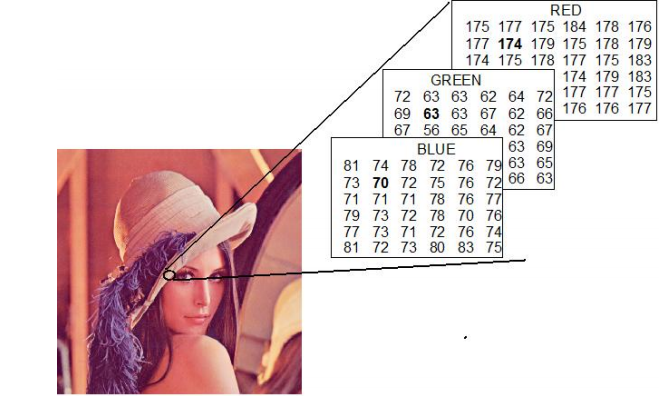
\includegraphics[width=7cm]{Imagens/colorida.png}
    \caption{Imagem Colorida}
    \label{fig:colorful}
\end{figure}

\begin{figure}[htp]
    \centering
    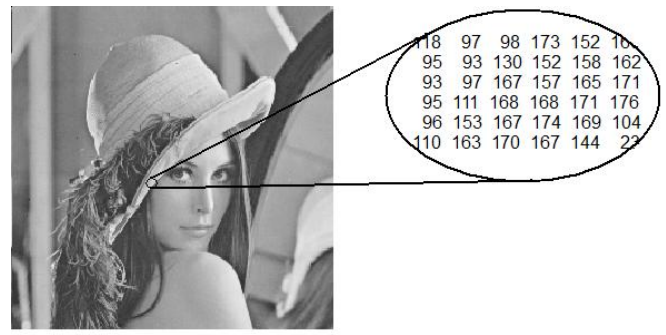
\includegraphics[width=6cm]{Imagens/gray.png}
    \caption{Imagem em GrayScale}
    \label{fig:gray}
\end{figure}


Já na figura \ref{fig:equal} no lado esquerdo está a imagem original já em \textit{GrayScale} antes da normalização dos níveis de seus pixels. E no lado direito, a imagem já foi equalizada e conta agora com uma maior nitidez ou pouca disparidade nos níveis dos pixels. 

\begin{figure}[h]
    \centering
    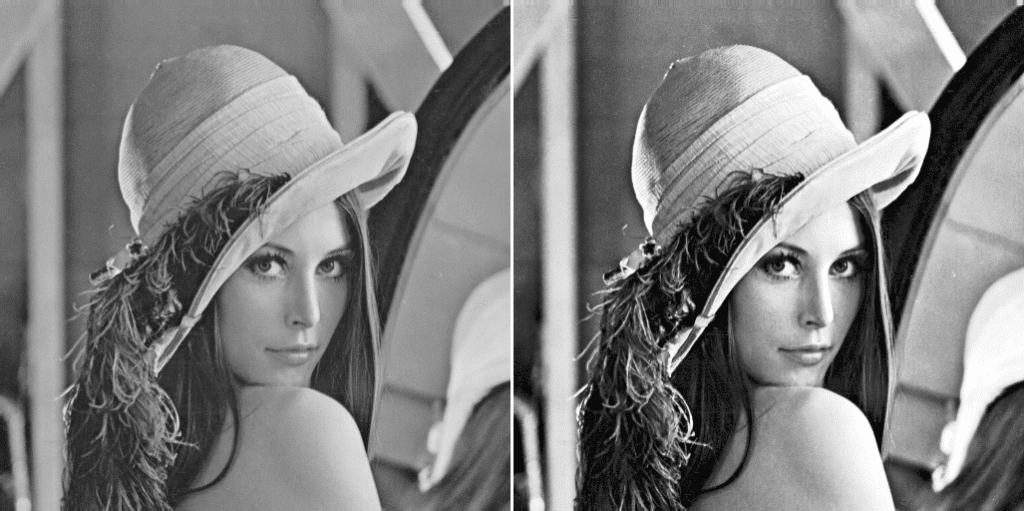
\includegraphics[width=6cm]{Imagens/lena_gray_eq-1024x511.png}
    \caption{Resultado do Histograma de Equalização}
    \label{fig:equal}
\end{figure}

\subsection{Execução dos Algoritmos}
\label{sub:alg_ex}
Após essa etapa descrita em \ref{sub:app_pross}, os algoritmos de Redes Neurais Convolucionais utilizando TensorFlow, SVM, KNN, Naive Bayes e Decision Tree foram executados para a base de dados devidamente pré-processada. 


\section{Análise de Resultados}
    Os resultados preliminares para o Cehckpoint 1 descritos na tabela \ref{tab:prem_result}, nela estão os valores de acurácia, métrica escolhida neste trabalho para avaliar a eficiência dos algoritmos citados anteriormente em classificar as imagens de lixo orgânico ou reciclável.
    
%\begin{table}[h]
%\centering
%\begin{tabular}{lrr}
%\toprule
%Scenario  & $\delta$ (s) & Runtime (ms) \\
%\midrule
%Paris       & 0.1  & 13.65      \\
%            & 0.2  & 0.01       \\
%New York    & 0.1  & 92.50      \\
%Singapore   & 0.1  & 33.33      \\
%            & 0.2  & 23.01      \\
%\bottomrule
%\end{tabular}
%\caption{Booktabs table}
%\label{tab:booktabs}
%\end{table}
    
    
\begin{table}[h]
\centering
\begin{tabular}{c|c|c|c|c|c|c|}
\cline{2-7}
\multicolumn{1}{l|}{}                 & \textbf{TF} & \textbf{SVM} & \textbf{KNN} & \textbf{NB} & \textbf{DT} & \textbf{RNA} \\ \hline
\multicolumn{1}{|c|}{\textbf{1ª}} & 50,0\%      & 68,0\%       & 61,55\%      & 57,75\%     & 57,99\%     & -            \\ \hline
\multicolumn{1}{|c|}{\textbf{2ª}} & 50,7\%      & 67,65\%      & 61,9\%       & 58,15\%     & 60,55\%     & -            \\ \hline
\multicolumn{1}{|c|}{\textbf{3ª}} & 50,0\%      & 67,75\%      & 60,9\%       & 57,49\%     & 60,3\%      & -            \\ \hline
\multicolumn{1}{|l|}{\textbf{M}}  & 50,2\%      & 67,8\%       & 61,45\%      & 57,79\%     & 59,6\%      & -            \\ \hline
\end{tabular}
\caption{Tabela de Resultados Preliminares}
\label{tab:prem_result}
\end{table}
    
\subsubsection{References}

The references section is headed ``References'', printed in the same
style as a section heading but without a number. A sample list of
references is given at the end of these instructions. Use a consistent
format for references. The reference list should not include publicly unavailable work.

\subsection{Citations}

Citations within the text should include the author's last name and
the year of publication, for example~\cite{gottlob:nonmon}.  Append
lowercase letters to the year in cases of ambiguity.  Treat multiple
authors as in the following examples:~\cite{abelson-et-al:scheme}
or~\cite{bgf:Lixto} (for more than two authors) and
\cite{brachman-schmolze:kl-one} (for two authors).  If the author
portion of a citation is obvious, omit it, e.g.,
Nebel~\shortcite{nebel:jair-2000}.  Collapse multiple citations as
follows:~\cite{gls:hypertrees,levesque:functional-foundations}.
\nocite{abelson-et-al:scheme}
\nocite{bgf:Lixto}
\nocite{brachman-schmolze:kl-one}
\nocite{gottlob:nonmon}
\nocite{gls:hypertrees}
\nocite{levesque:functional-foundations}
\nocite{levesque:belief}
\nocite{nebel:jair-2000}




%% The file named.bst is a bibliography style file for BibTeX 0.99c
\bibliographystyle{named}
\bibliography{ijcai21}

\end{document}

